\documentclass[Report.tex]{subfiles}

\begin{document}

\chapter{Discussion}

\section{Result of the \textit{LTEWatch} Project}
\;\\[-50pt]
\begin{figure}[H]
	\centering
	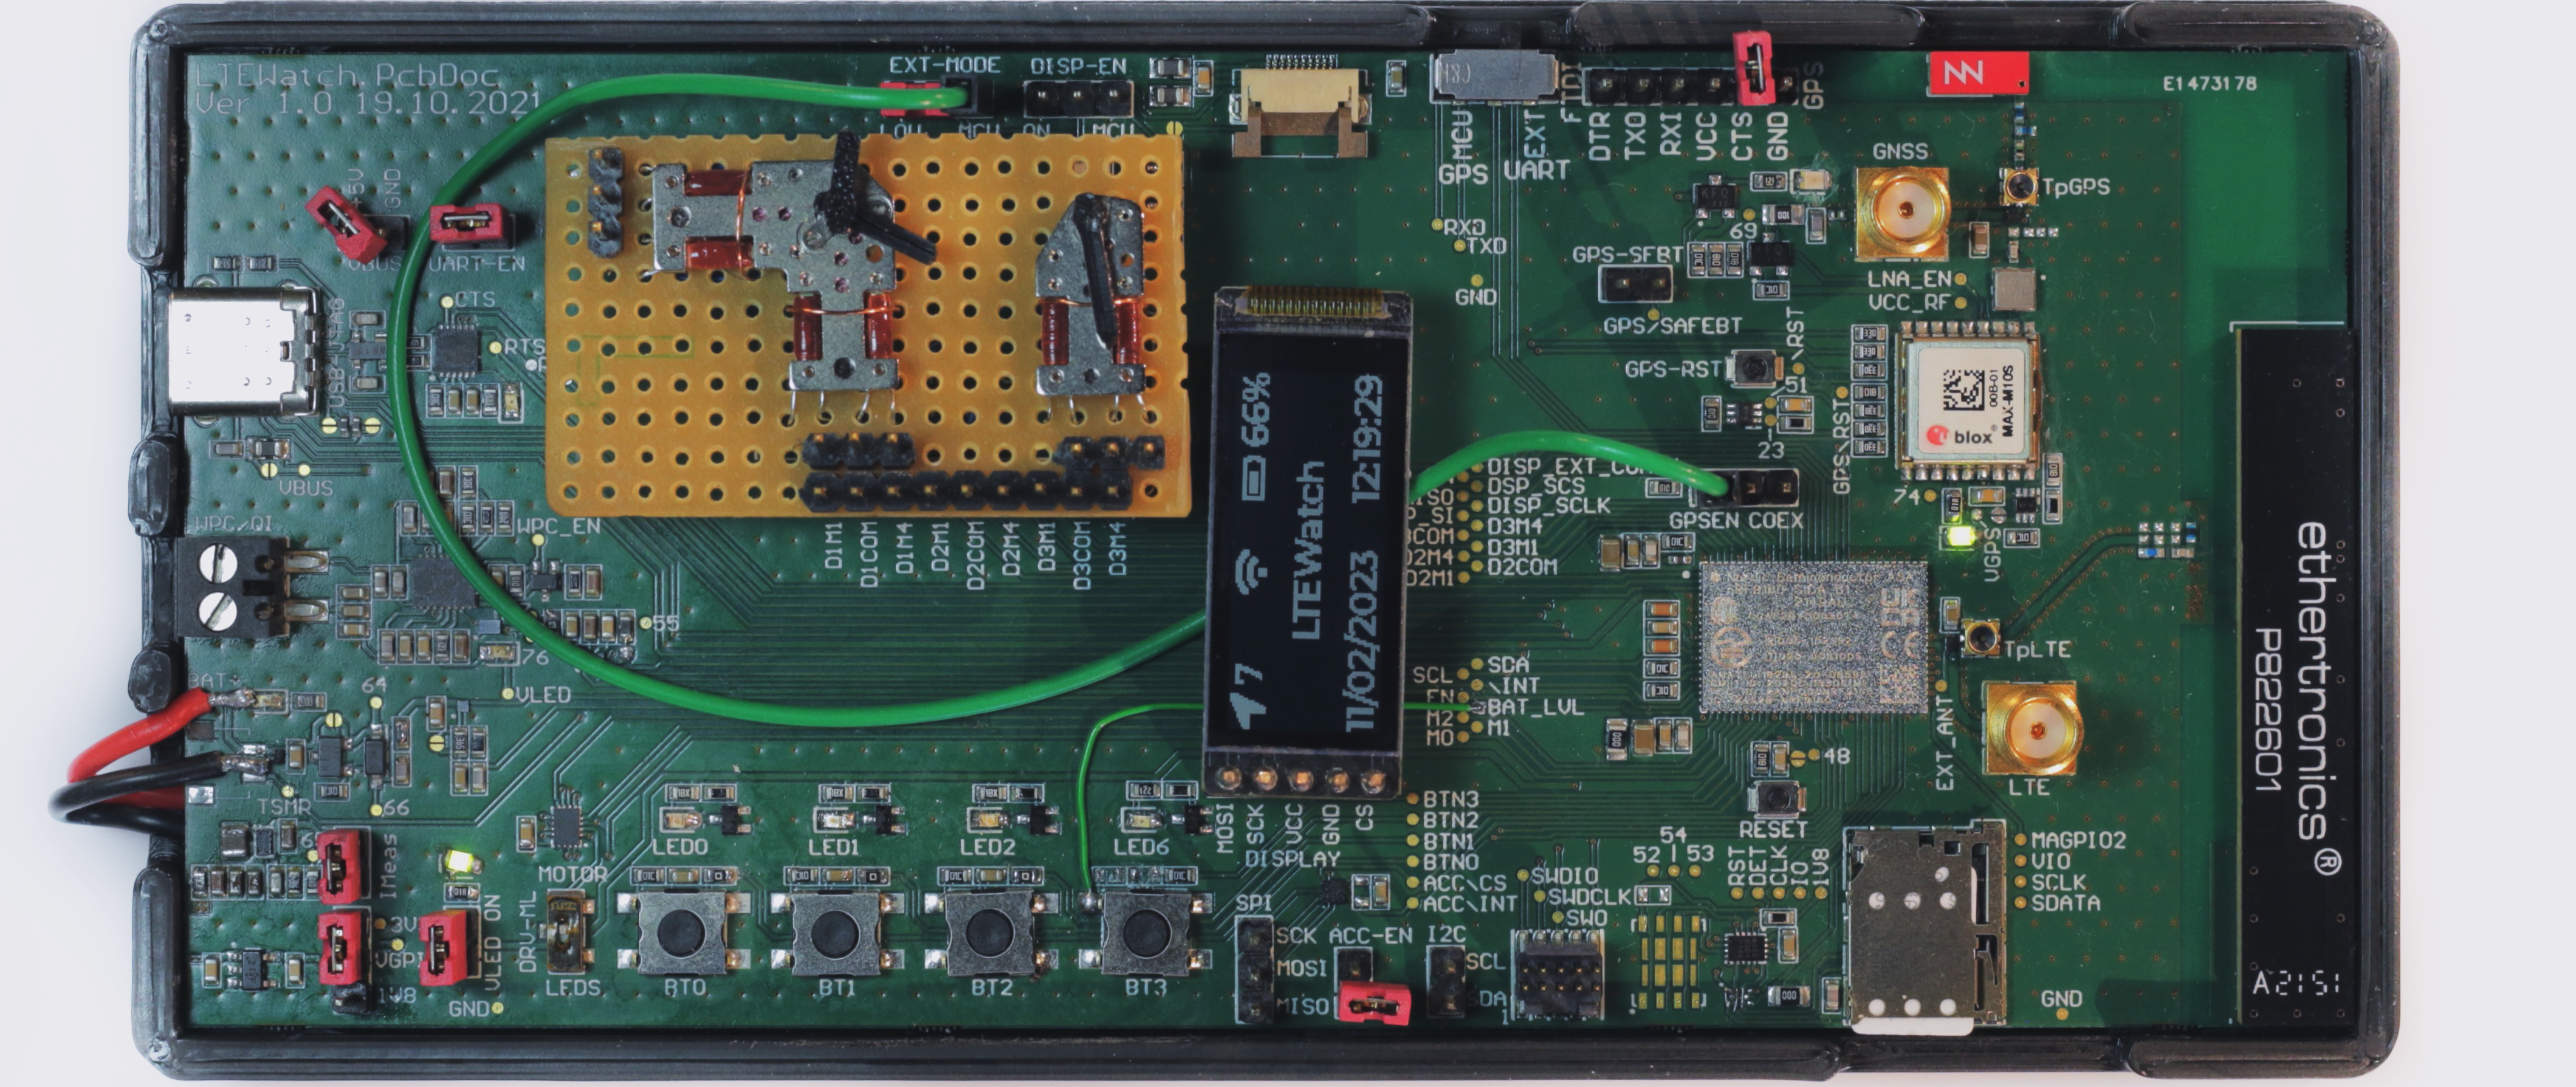
\includegraphics[width=1\textwidth]{Include/Figure/LTEWatch_img/ltewatch_img_1_1.png}
	\caption{\textit{LTEWatch} Prototype Device}
	\label{fig:ltewatch_img_1_1}
\end{figure}

It is now time to make the point on the project that has been carried out. Firstly, this work was a very complex and complete project which required a very varied panoply of skills by covering all steps of a device prototype design and realization. At the end of the project, a functional prototype board «LTEWatch» have been designed, built and validated.\\

Figure \ref{fig:ltewatch_img_2} illustrates the \textit{LTEWatch} prototype device that was made for this Master Thesis Project:

\begin{figure}[H]
	\centering
	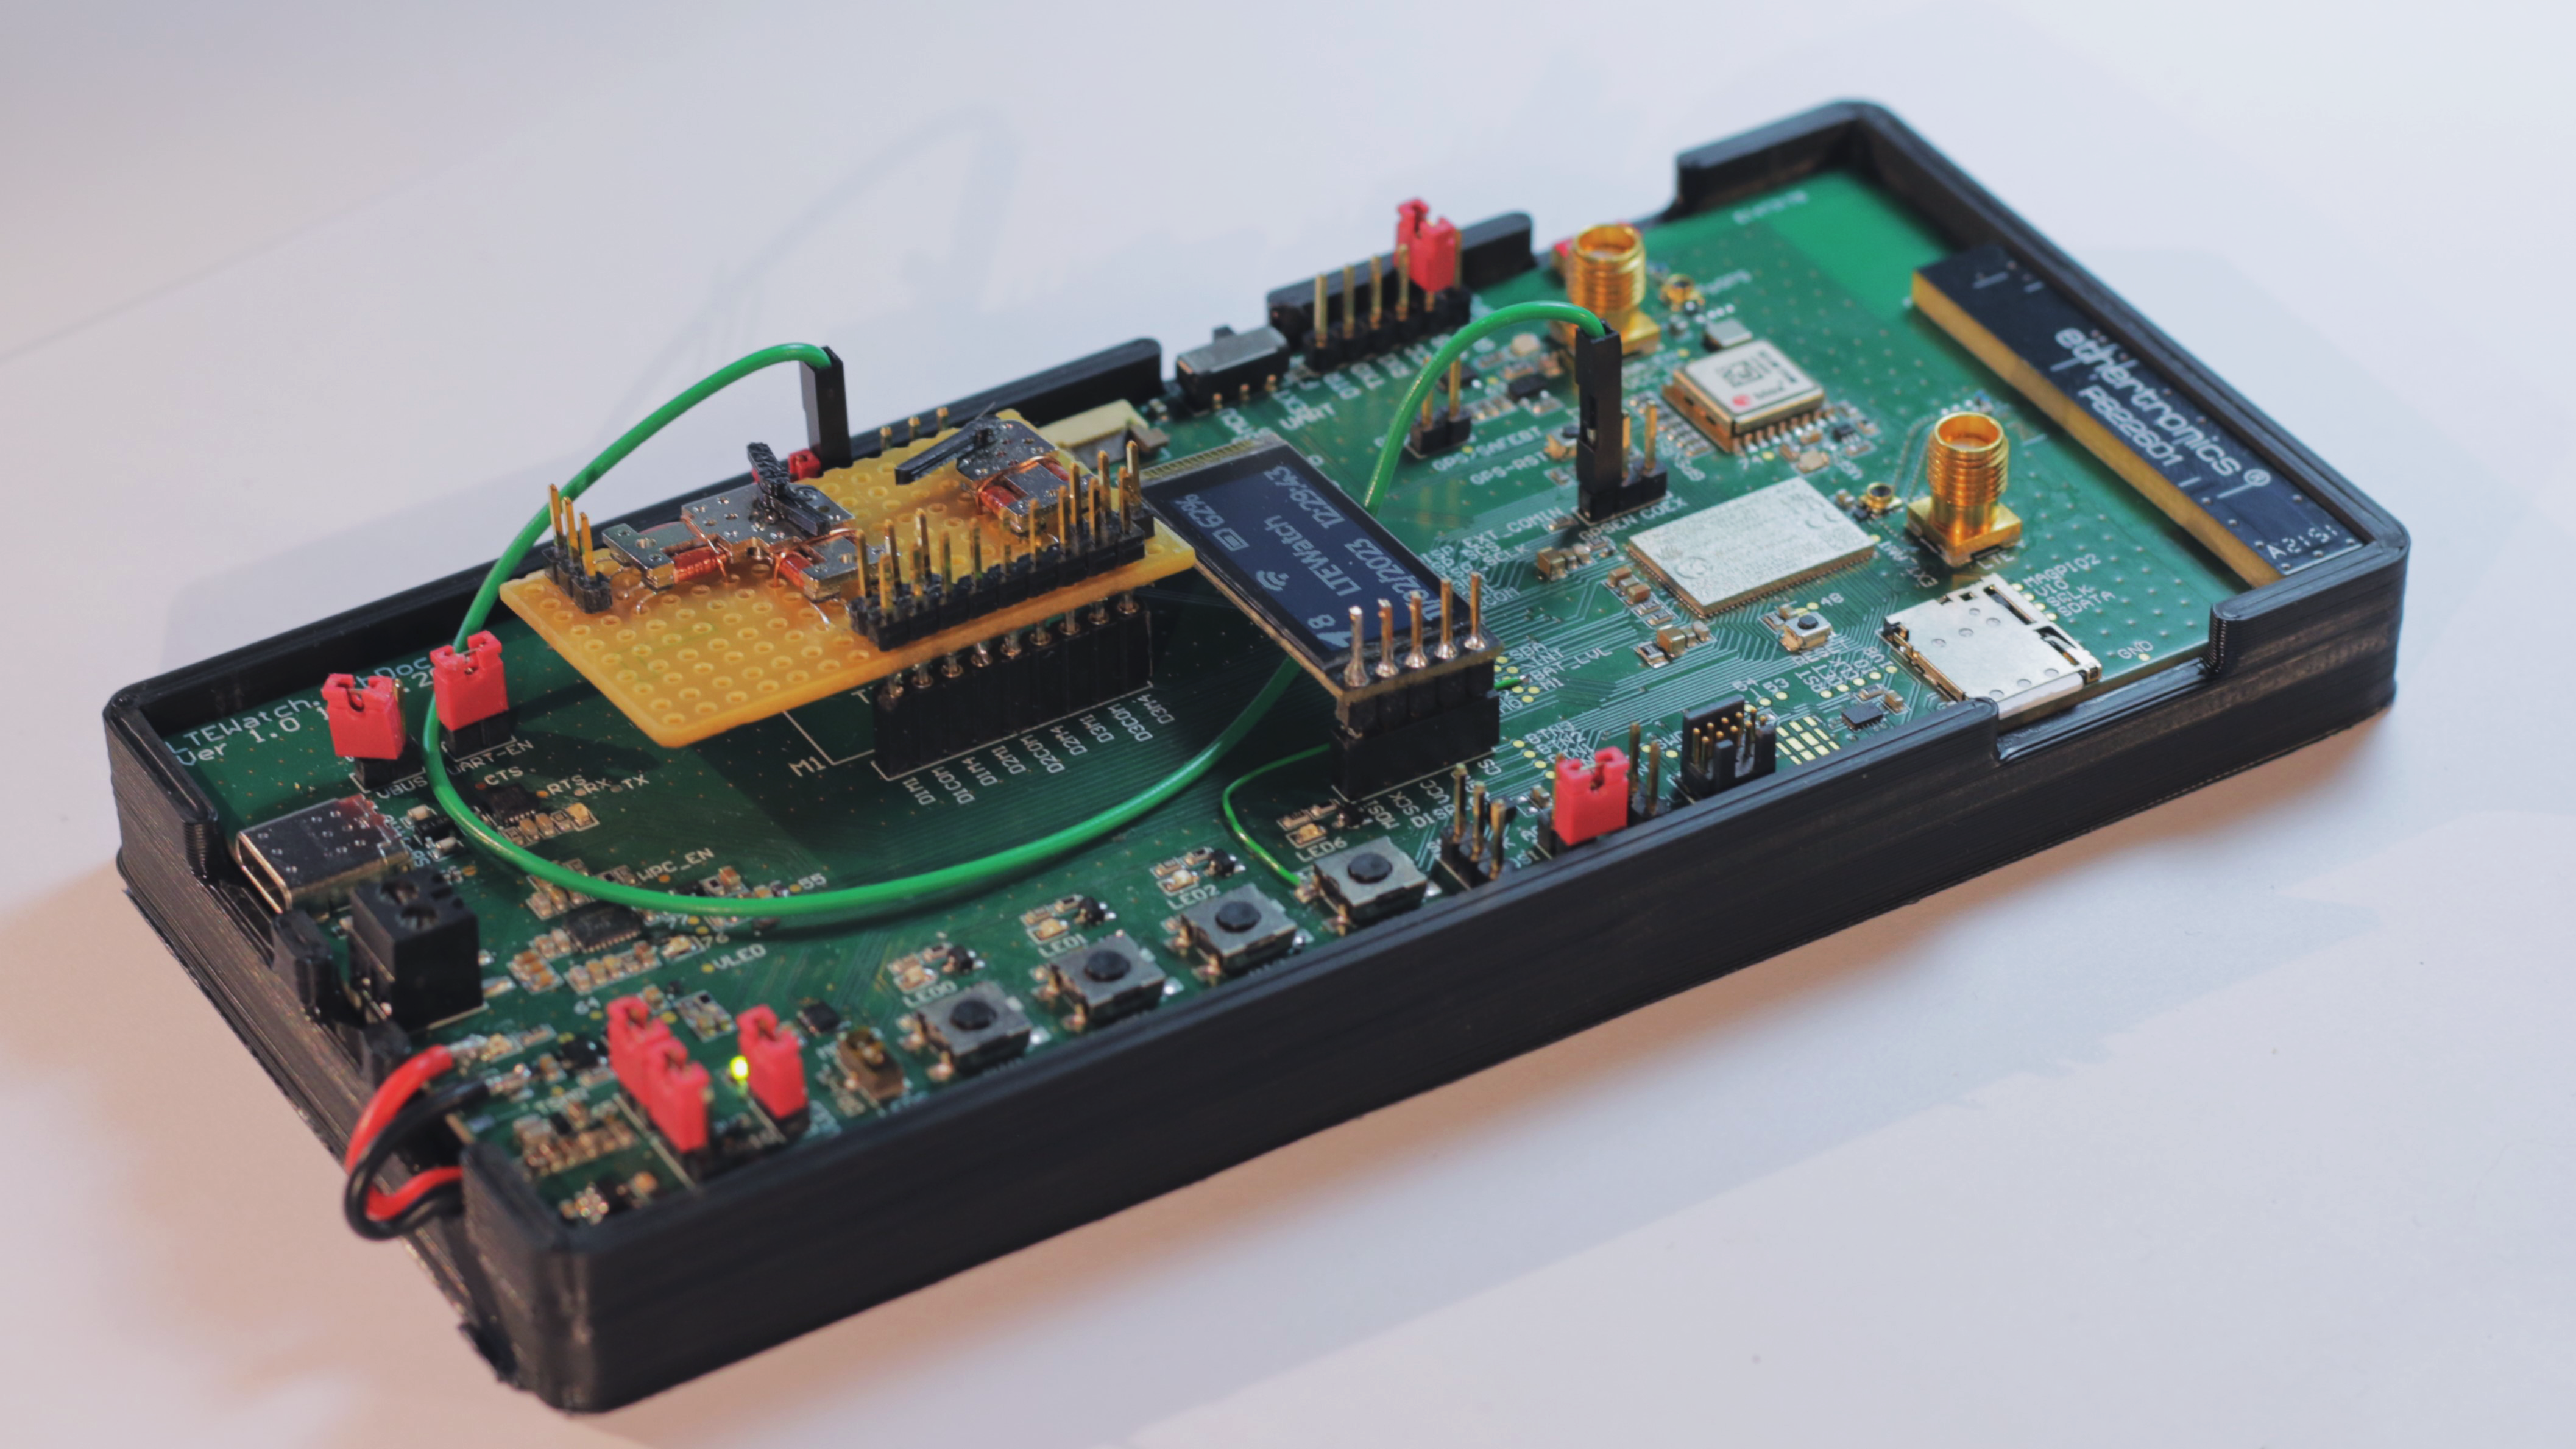
\includegraphics[width=0.9\textwidth]{Include/Figure/LTEWatch_img/ltewatch_img_2.png}
	\caption{\textit{LTEWatch} Prototype Device}
	\label{fig:ltewatch_img_2}
\end{figure}

The finished \textit{LTEWatch} prototype device validates the following features:
\begin{enumerate}
\item \textbf{Power Supply:}
\begin{itemize}
\item Recharge by \textit{USB-C}
\item Suitable for \textit{Li-Ion} and \textit{LiPo} single cell batteries with programmable battery manager
\item Battery level monitoring and displaying
\item \textit{WPC/QI} wireless battery charging capability
\end{itemize}
\item \textbf{User Interface:}
\begin{itemize}
\item Display hour, minute and second using tiny stepper motors
\item Four fully programmable push button to operate the device
\item Graphical interface using an ultra-low-power \textsc{SHARP} \textit{Memory-In-Pixel (MIP) LCD}
\item 3-axis ultra-low-power \textit{MC3635} accelerometer from \textsc{mCube}
\end{itemize}
\item \textbf{\textit{GNSS}:}
\begin{itemize}
\item \textit{GNSS} tracking using \textit{MAX-M10S} ultra-low-power \textit{GNSS} receiver from \textsc{u-blox}
\item Selectable external antenna via SMA or on-board \textit{DUO mXTEND (NN03-320)} from \textsc{igion}
\end{itemize}
\item \textbf{\textit{LTE-M/NB-IoT}:}
\begin{itemize}
\item Selectable external antenna via \textit{SMA} or on-board \textit{P822601} antenna from \textsc{Kyocera}
\item Data publishing on a \textit{ThingsBoard} server by \textit{LTE-M/NB-IoT} using \textit{MQTT} protocol
\item Connector for \textit{SIM} and \textit{eSIM} card
\end{itemize}
\end{enumerate}

\pagebreak

\section{Remaining Work and Further Improvement}

Due to the relatively limited time available for this project, it was only possible to dedign a prototype board of \textit{LTEWatch} and even if most of the specifications were implemented it still remains some tasks that should be finished:
\begin{enumerate}
\item \textbf{Accelerometer:}
\begin{itemize}
\item Find a \textit{Zephyr} compatible driver for the \textit{MC3635} accelerometer
\item Implement accelerometer functionality in \textit{LTEWatch} firmware
\item Implement accelerometer wake-up function and activity tracking features
\end{itemize}
\item \textbf{\textit{LTE-M/NB-IoT} Custom Antenna:}
\begin{itemize}
\item Look for an antenna design solution such as an antenna integrated in the watch strap or in the case
\item Design and simulate a custom antenna solution
\item Test custom solution performance
\end{itemize}
\item \textbf{Power Management and Consumption:}
\begin{itemize}
\item Implement low power and power management features from \textit{Zephyr} and \textit{nRF Connect SDK}
\end{itemize}
\item \textbf{Bluetooth \& Wifi:}
\begin{itemize}
\item Integrate the \textit{nRF52840} in the hardware design to add \textit{bluetooth} and \textit{Wifi} features for improved connectivity
\end{itemize}
\item \textbf{Round PCB:}
\begin{itemize}
\item Clean \textit{LTEWatch} hardware design by removing all unnecessary modules and components
\item Root a compact round PCB for a smart-watch design
\end{itemize}
\item \textbf{Mechanical:}
\begin{itemize}
\item Design a \textit{3D} printed case for the round PCB
\item Design a watch strap solution that can integrate a custom antenna
\end{itemize}
\end{enumerate} 

\end{document}

